%%%%%%%%%%%%%%%%%%%%%%%%%%%%%%%%%%%%%%%%%
% University/School Laboratory Report
% LaTeX Template
% Version 3.1 (25/3/14)
%
% This template has been downloaded from:
% http://www.LaTeXTemplates.com
%
% Original author:
% Linux and Unix Users Group at Virginia Tech Wiki 
% (https://vtluug.org/wiki/Example_LaTeX_chem_lab_report)
%
% License:
%  CC BY-NC-SA 3.0 (http://creativecommons.org/licenses/by-nc-sa/3.0/)
%
%%%%%%%%%%%%%%%%%%%%%%%%%%%%%%%%%%%%%%%%%

%---------------------------------------------------------------------
% 	PACKAGES AND DOCUMENT CONFIGURATIONS
%-------------------------------------------------------------------

\documentclass{report}
\usepackage[utf8]{inputenc}
\usepackage[left=2.50cm, right=1.00cm, top=1.00cm, bottom=2.00cm]{geometry}
\usepackage{siunitx} % Provides the \SI{}{} and \si{} command for typesetting SI units
\usepackage{graphicx} % Required for the inclusion of images
\usepackage{caption}
\usepackage{subcaption}
\usepackage{natbib} % Required to change bibliography style to APA
\usepackage{amsmath} % Required for some math elements 
\usepackage{amssymb}
\usepackage{blindtext}
\usepackage{tikz}
\usetikzlibrary{matrix}
%\setlength\parindent{0pt} % Removes all indentation from paragraphs
\usepackage[framed]{matlab-prettifier}
\definecolor{mygreen}{RGB}{28,172,0} % color values Red, Green, Blue
\definecolor{mylilas}{RGB}{170,55,241}
\usepackage{listings}
\lstset{
	style=Matlab-editor,
	basicstyle         = \fontsize{8}{11}\ttfamily,
	numberstyle       =\fontsize{8}{11}\ttfamily,
	%backgroundcolor=\color{gray},
	%mlshowsectionrules = true,
	rangeprefix        = \%\ 
}

\renewcommand{\labelenumi}{\alph{enumi}.} % Make numbering in the enumerate environment by letter rather than number (e.g. section 6)

%\usepackage{times} % Uncomment to use the Times New Roman font
%-------------------------------------------------------------------
% 	TITLE PAGE
%-------------------------------------------------------------------
% Title Page
\title{TIC}
\author{Mauricio Caceres}
\date{18 décembre 2016}

%-------------------------------------------------------------------
% 	DOCUMENT INFORMATION
%-------------------------------------------------------------------

\begin{document}
\begin{titlepage}
	\centering
	\vfill
{\bfseries\huge Communication sans fil}
	\vfill
	{\bfseries\LARGE
		TP:\\
		Code division multiple acces \\capacité du canal
		\\
		\vskip2cm

		Master SISEA\\
	
	}
	\vfill
	18 décembre 2016
	\vfill
	{\large Mauricio Caceres } \hfill  {\large Enseignant : Pascal Scalart}
	\vfill
	
\includegraphics[width=9cm]{rennes} % also works with logo.pdf    
	\vfill
	
\includegraphics[width=6cm]{enssat} % also works with logo.pdf
	\vfill
	\vfill
\end{titlepage}
\tableofcontents

%\begin{center}
%\begin{tabular}{l r}
%Date Performed: & January 1, 2012 \\ % Date the experiment was performed
%Partners: & James Smith \\ % Partner names
%& Mary Smith \\
%Instructor: & Professor Smith % Instructor/supervisor
%\end{tabular}
%\end{center}


% If you wish to include an abstract, uncomment the lines below
% \begin{abstract}
% Abstract text
% \end{abstract}

%-------------------------------------------------------------------
% 	SECTION 1
%-------------------------------------------------------------------
\chapter{Introduction}%7
%RE REDIGER CETTE SECTION POUR LA FAIRE PAS COMME ICI
Du fait du codage spécifique autorisant une bande passante élargie, les techniques d’étalement
de spectre possèdent des propriétés spécifiques différentes de celles des signaux faible bande.
Ces techniques ouvrent notamment la possibilité d’accées multiples . Si plusieurs utilisateurs
transmettent au même moment des signaux modulés par étalement de spectre, le récepteur
peut distinguer ces différents utilisateurs à condition que chacun d’entre eux possède un code
d’étalement unique ayant des propriétés de faible intercorrélation avec les autres mots de
codes utilisés.
Si l’on effectue, au niveau du récepteur, la corrélation entre le signal reçu et un code
d’étalement utilisé par un utilisateur, le signal provenant de cet utilisateur sera des-étalé tandis
que les signaux provenant des autres utilisateurs resteront étalés sur une large bande
passante.

\section{Définitions et concepts utilises}%8
%CHANGER LES DESCRIPSION DE LES DEFINITIONS
\begin{description}
	\item  [Label 1] Le texte de cette etiquette est le suivante
\end{description}

%------------------------------------------------------------------
% 	SECTION 2
%-----------------------------------------------------------------
\chapter{Implementation en Matlab/Simulink}%1
\section{Etude de l'étalement de spectre}%2
Dans cette section on va étudier l'effet de la codification et son impact dans la forme du spectre.
La codification est faite en multipliant élément par élément le code par la signal. Dans la Fig.\ref{fig:schemaq1} le schéma de contruction dans le 
logiciel Simulink.
\begin{figure}[h]
	\centering
	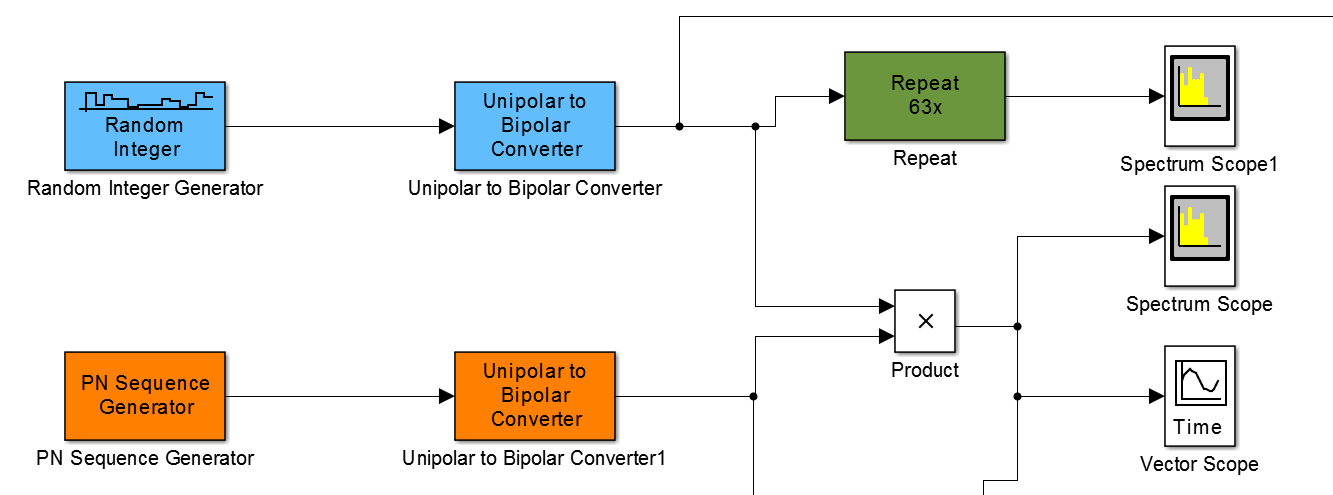
\includegraphics[width=0.7\linewidth]{schema_q1_solo_63}
	\caption{shema q1}
	\label{fig:schemaq1_solo}
\end{figure}

D'abord on genere la signal à étudier avec une suite aleatoire de entier entre 0 et 1 pour après 
convertir cette signal en bipolaire, c'est à dire valeur entre -1 et 1. Cela est
fait pour que la multiplication élément par élément avec le code soit cohérente.\\%AGREGAR ALGUN QUE OTRO DETALLE AQUI

Ensuite la génération du code a lieu dans la voie inférieur de la Fig.\ref{fig:schemaq1_solo}
un générateur de code pseudo aléatoire %SE PUEDE EXPLICAR COMO FUNCIONA EL GENERADOR ALEATORIO ACA ABAJO ESTA LA INFO
%Generate a pseudorandom noise (PN) sequence using a linear feedback shift register (LFSR). The LFSR is implemented using a simple shift register generator (SSRG, or Fibonacci) configuration.
%
%The 'Generator polynomial' parameter values specify the shift register connections. Enter these values as either a binary vector or a descending-ordered polynomial. For the binary vector representation, the first and last elements of the vector must be 1. For the descending-ordered polynomial representation, the last element of the vector must be 0.
%
%The 'Output mask source' may be from a dialog parameter or an input port. The 'Output mask vector' is a binary vector corresponding to the shift register states that are to be XORed to produce the output sequence values. Alternatively, you may enter an integer 'scalar shift value' to produce an equivalent advance or delay in the output sequence.
%
%For variable-size output signals, the current output size is either specified from the 'oSiz' input or inherited from the 'Ref' input.
%



\subsection{Observation dans le domaine temporel}

La signal est observé dans le domaine temporel après d'être multiplie par le code pour bien vérifier au moment 
de la réception que les données on était bien reçu. Malheureusement la simulation ne permet pas de voir les premières
instant pour faire une validation en regardant les premières données obtenues.

\begin{figure}[h]
	\centering
	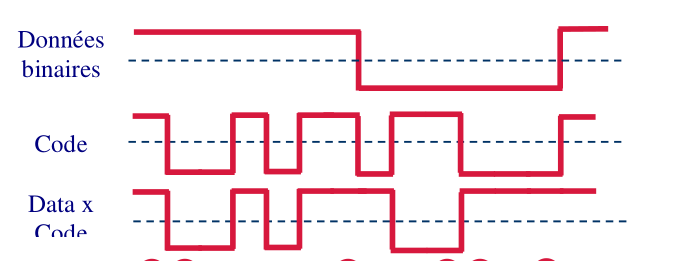
\includegraphics[width=0.5\linewidth]{error_rojo}
	\caption{En regardant les graph temporel on peut vérifier si le codage est fait correctement}
	\label{fig:errorrojo}
\end{figure}

Pourtant nous ferons après le calcul de l'erreur et nous pourrons constater que la signal arrive correctement au récepteur.\\
L'observation de la signal dans le domaine temporel par le bias du "vector scope" est montré dans la Fig \ref{fig:temporelq1decodificada} et la Fig \ref{fig:temporelq1codificada} ce sont bien des valeur entre 



 En sortie du codificador la simulation nous montre cette suite de point généres de manières aléatoires.
 
%\begin{figure}[h]
%	\centering
%	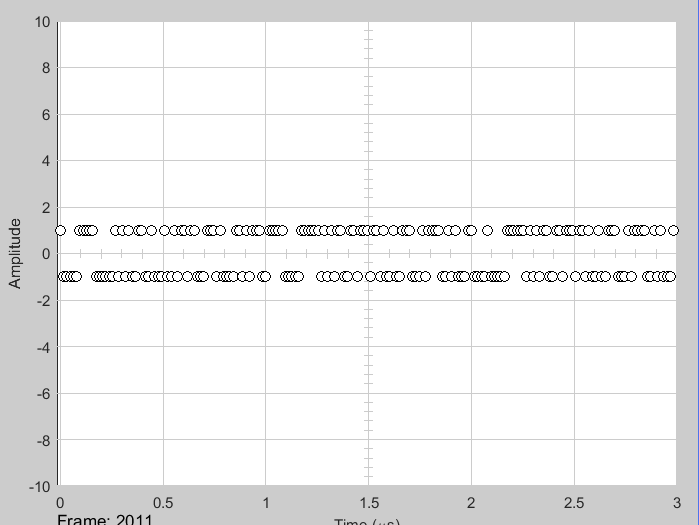
\includegraphics[width=0.7\linewidth]{temporel_q1_codificada}
%	\caption{signal codificada}
%	\label{fig:temporelq1codificada}
%\end{figure}
%
%\begin{figure}[h]
%	\centering
%	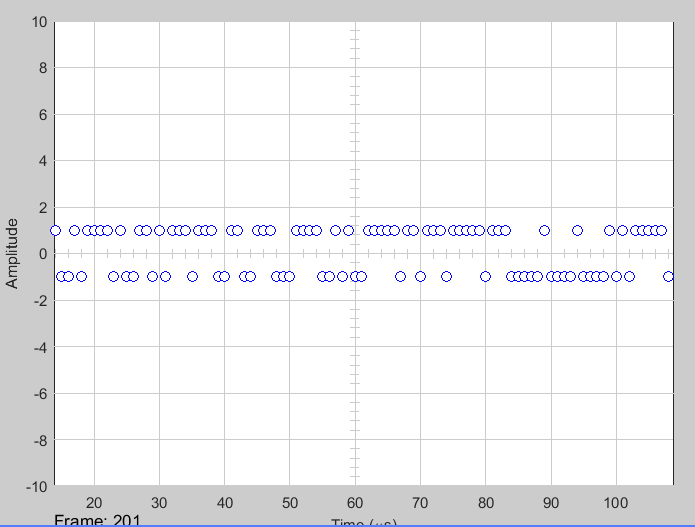
\includegraphics[width=0.7\linewidth]{temporel_q1_decodificada}
%	\caption{signal codificada}
%	\label{fig:temporelq1decodificada}
%\end{figure}

\begin{figure}
	\centering
	\begin{subfigure}[b]{0.4\textwidth}
		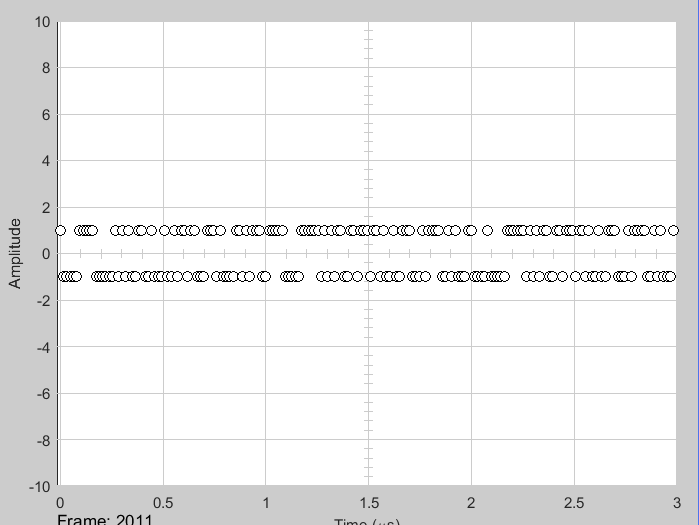
\includegraphics[width=\textwidth]{temporel_q1_codificada}
			\caption{signal en sortie du codeur}
		\label{fig:temporelq1codificada}
	\end{subfigure}
	~ %add desired spacing between images, e. g. ~, \quad, \qquad, \hfill etc. 
	%(or a blank line to force the subfigure onto a new line)
	\begin{subfigure}[b]{0.4\textwidth}
		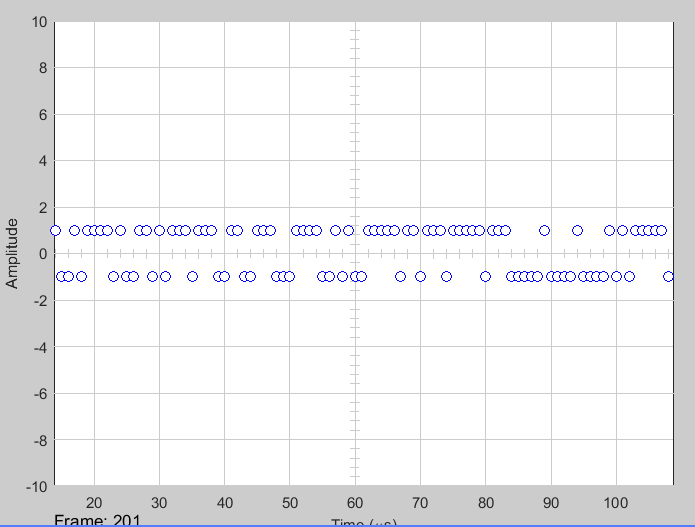
\includegraphics[width=\textwidth]{temporel_q1_decodificada}
			\caption{signal en sortie du décodeur}
		\label{fig:temporelq1decodificada}
	\end{subfigure}
\end{figure}



\subsection{Observation dans le domaine fréquenciel}

L'spectre du signal générée avant et après la fonction multiplication pour un valeur de n = 7 et du vecteur de 
polynome générateur $ [1 1 0 0 0 0 1] $ (après nous analyserons l'effet de changer cette paramètre).\\


\begin{figure}[h]
	\centering
	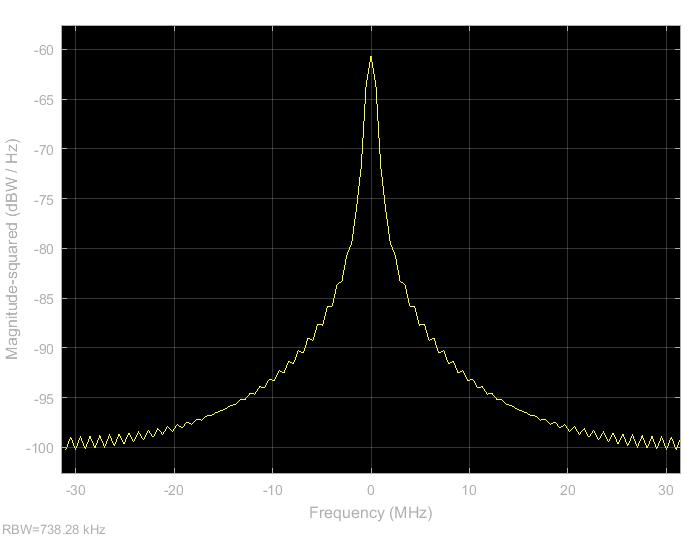
\includegraphics[width=0.7\linewidth]{cdma_2_jpg}
	\caption{something}
	\label{fig:cdma2jpg}
\end{figure}

%\begin{figure}
%	\centering
%	\begin{subfigure}[b]{0.4\textwidth}
%	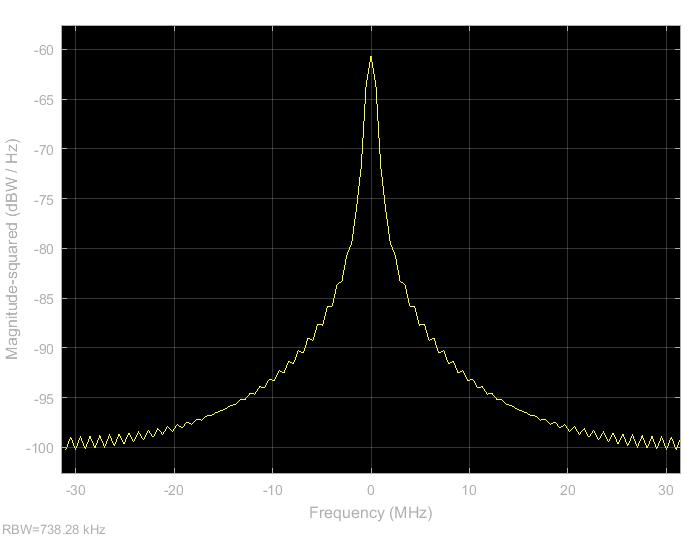
\includegraphics[width=0.9\linewidth]{cdma_2_jpg}
%\caption{something}
%\label{fig:cdma2jpg}
%	\end{subfigure}
%	~ %add desired spacing between images, e. g. ~, \quad, \qquad, \hfill etc. 
%	%(or a blank line to force the subfigure onto a new line)
%	\begin{subfigure}[b]{0.4\textwidth}
%	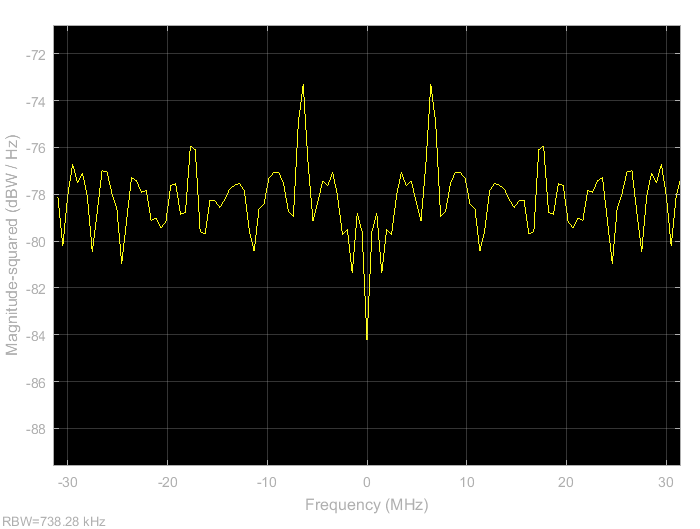
\includegraphics[width=0.9\linewidth]{cdma_1_jpg}
%\caption{something}
%\label{fig:cdma1jpg}
%	\end{subfigure}
%\end{figure}


Dans la Fig \ref{fig:cdma1jpg} l'espectre n'est pas étale la puissance est concentrée dans une bande 20Mhz (-10Mhz à 10Mhz) en ayant une valeur de -60 dBW/Hz

\begin{figure}[h]
	\centering
	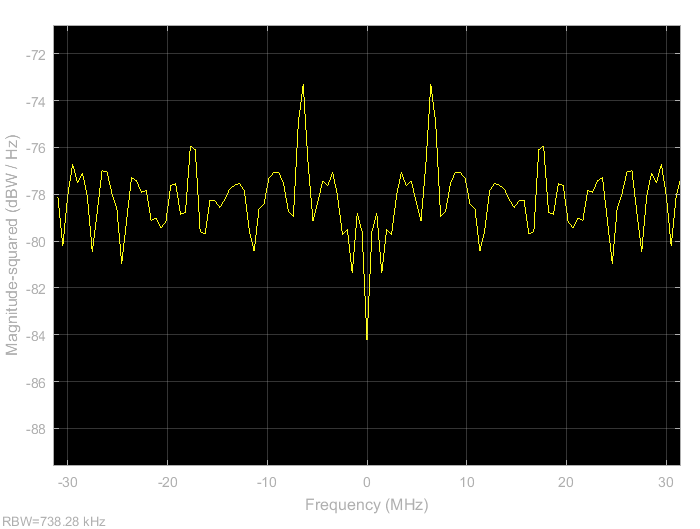
\includegraphics[width=0.6\linewidth]{cdma_1_jpg}
	\caption{something}
	\label{fig:cdma1jpg}
\end{figure}

Dans le cas du spectre de signal modifiée par le code la valeur maximale de la puissance diminue approximativement jusqu'à -74 dB/Hz  mais elle est repartie de manière plus uniforme sur tous les fréquences.

\subsection{Génération du polynome avec n=7 y n=3}

\subsubsection{n = 7}

On a changé le polynôme générateur pour voir les effets sur le spectre. Les résultats obtenues sont dans les Fig. \ref{fig:segundoespectroparan77} et la Fig. \ref{fig:segundospectroparan7} mais on peut conclure que pour le choix fait
il n'y a pas trop de différence par rapport au graph obtenues dans la Fig. \ref{fig:cdma2jpg} et la Fig. \ref{fig:cdma1jpg}.
%\begin{figure}[h]
%	\centering
%	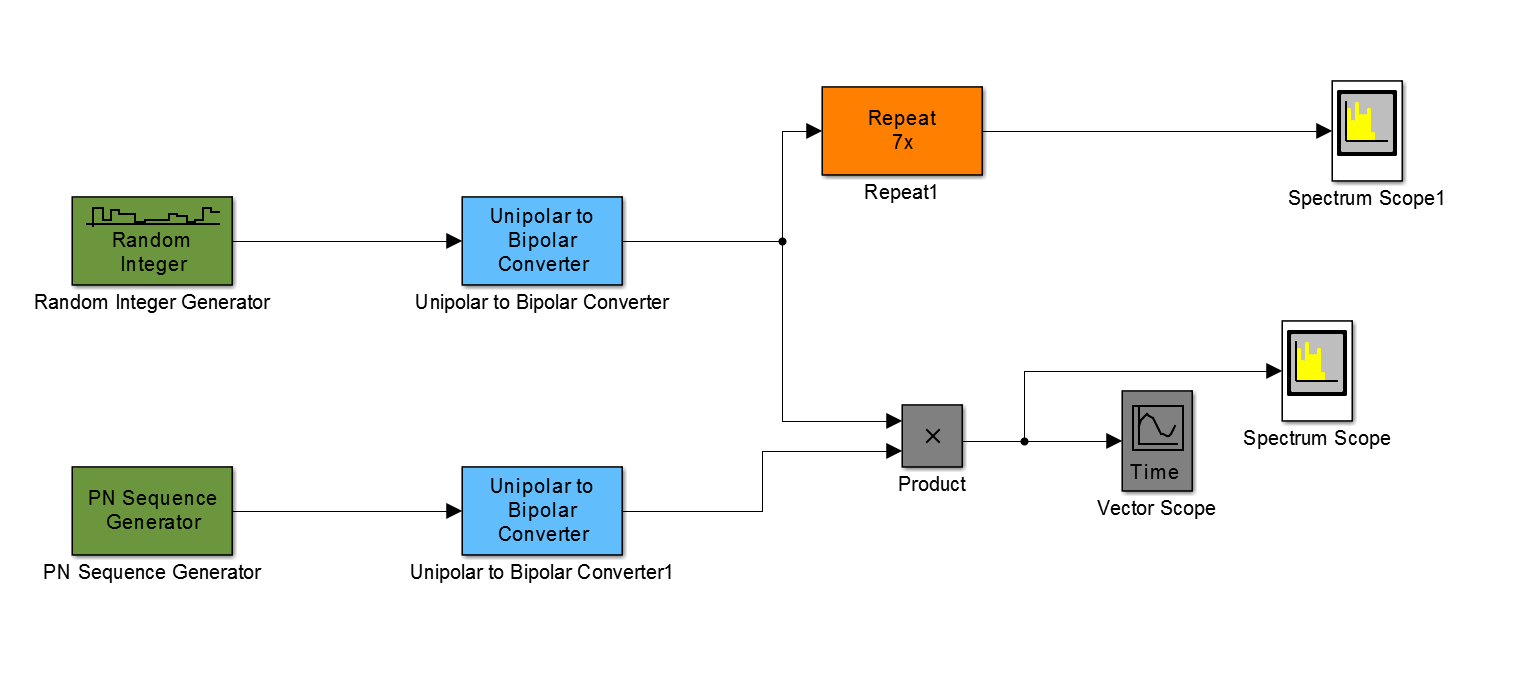
\includegraphics[width=0.9\linewidth]{schemanx77}
%	\caption{schema para nx7}
%	\label{fig:schemanx77}
%\end{figure}


\begin{figure}
	\centering
	\begin{subfigure}[b]{0.4\textwidth}
	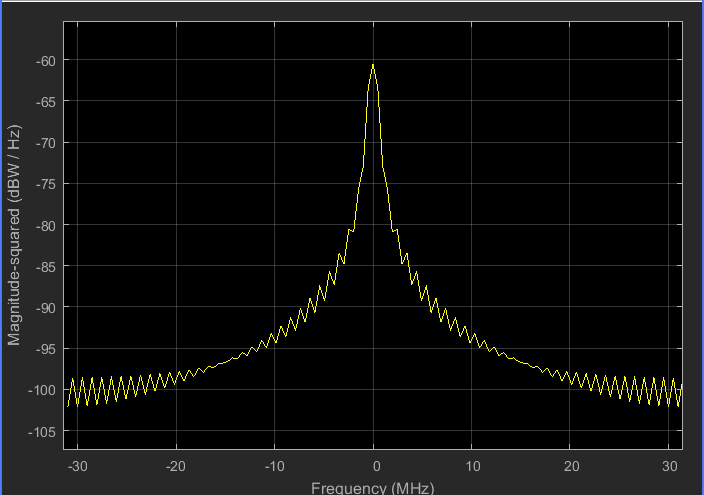
\includegraphics[width=0.9\linewidth]{segundo_espectro_paran77}
\caption{spectre para n = 7 avec une autre polynome generateur}
\label{fig:segundoespectroparan77}
	\end{subfigure}
	~ %add desired spacing between images, e. g. ~, \quad, \qquad, \hfill etc. 
	%(or a blank line to force the subfigure onto a new line)
	\begin{subfigure}[b]{0.4\textwidth}
	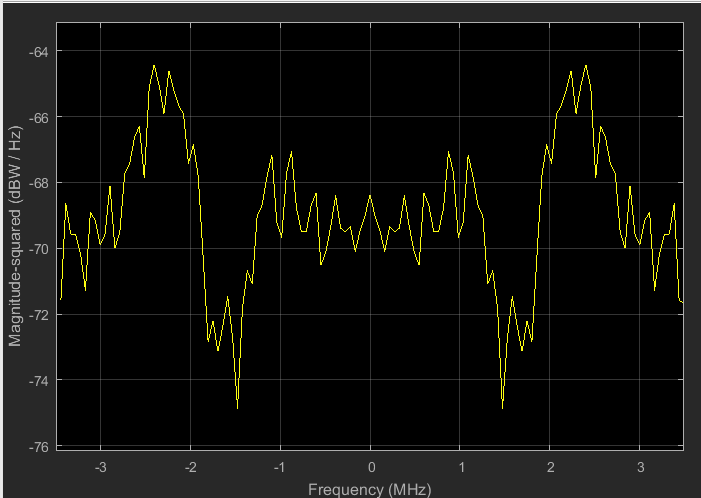
\includegraphics[width=0.9\linewidth]{segundo_spectro_paran7}
\caption{segundo spectreo para n = 7}
\label{fig:segundospectroparan7}
	\end{subfigure}
\end{figure}


%\begin{figure}[h]
%	\centering
%	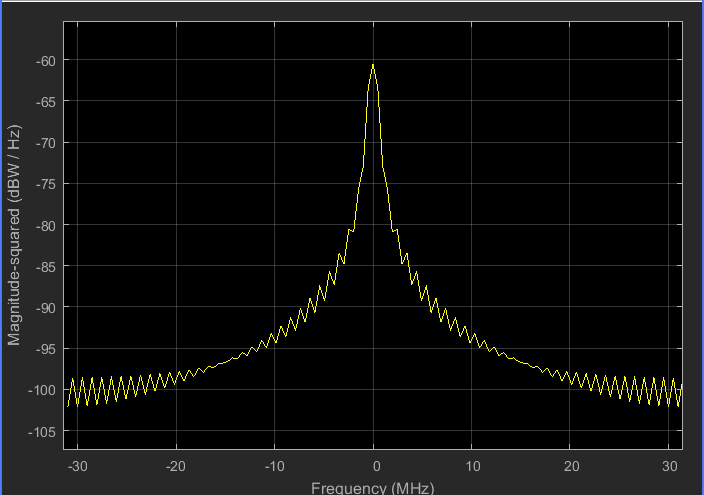
\includegraphics[width=0.9\linewidth]{segundo_espectro_paran77}
%	\caption{spectre para n = 7}
%	\label{fig:segundoespectroparan77}
%\end{figure}
%
%
%\begin{figure}[h]
%	\centering
%	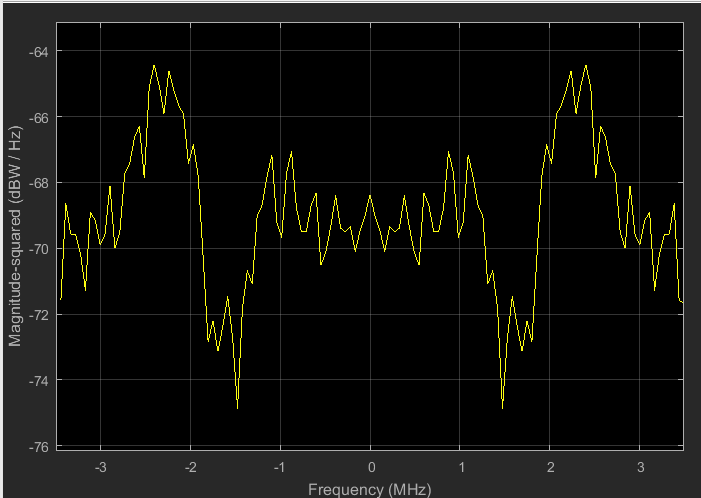
\includegraphics[width=0.9\linewidth]{segundo_spectro_paran7}
%	\caption{segundo spectreo para n = 7}
%	\label{fig:segundospectroparan7}
%\end{figure}


\subsubsection{n = 3}
Pour avoir une taille de polynôme générateur n = 3 il faut changer aussi le paramétré du blocs de répétition pour
faire un échantillonnage correctement. On voit cela dans la figure \ref{fig:schemaq1_solo_7}
\begin{figure}[h]
	\centering
	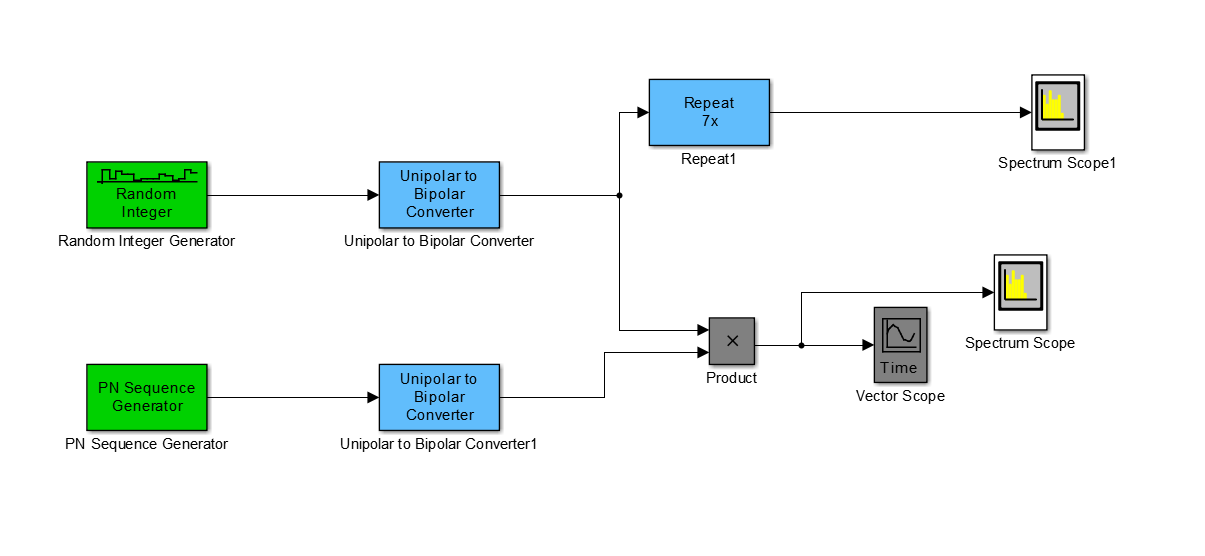
\includegraphics[width=0.6\linewidth]{schema_q1_solo}
	\caption{shema q1}
	\label{fig:schemaq1_solo_7}
\end{figure}
La observation dans le domaine de la fréquence obtenue avant de la modification du code (Fig. \ref{fig:spectren33}) 
montre moins de concentration de la puissance en ayant la même repartie dans autres fréquences mais tout en restant
plus concentrée dans ces fréquences. C'est ne pas le cas de la Fig. \ref{fig:spectren3} qui montre le étalement de spectre dans toutes les fréquences après la multiplication par le code.

%\begin{figure}[h]
%	\centering
%	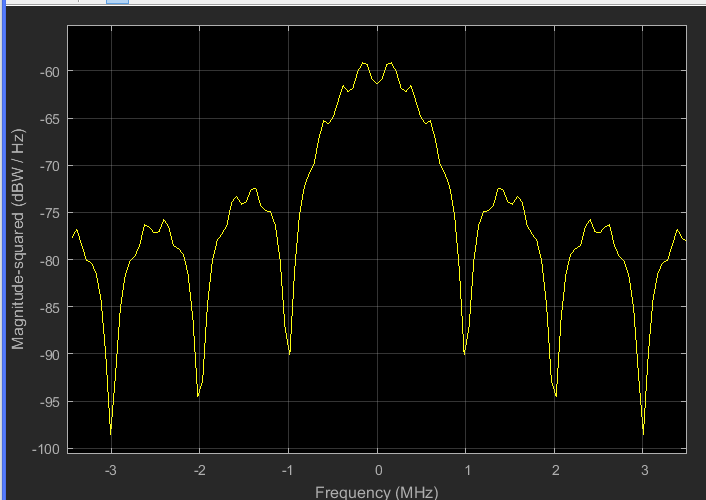
\includegraphics[width=0.6\linewidth]{spectren33}
%	\caption{spectre pour n = 3}
%	\label{fig:spectren33}
%\end{figure}
%
%\begin{figure}[h]
%	\centering
%	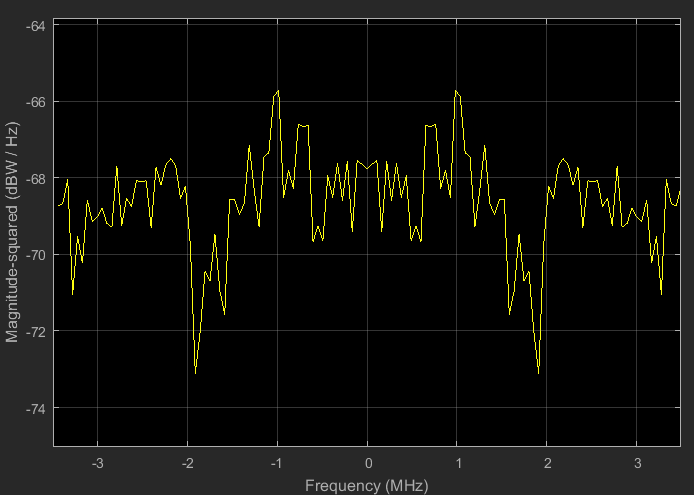
\includegraphics[width=0.6\linewidth]{spectren3}
%	\caption{spectre pour n = 3}
%	\label{fig:spectren3}
%\end{figure}


\begin{figure}
	\centering
	\begin{subfigure}[b]{0.4\textwidth}
	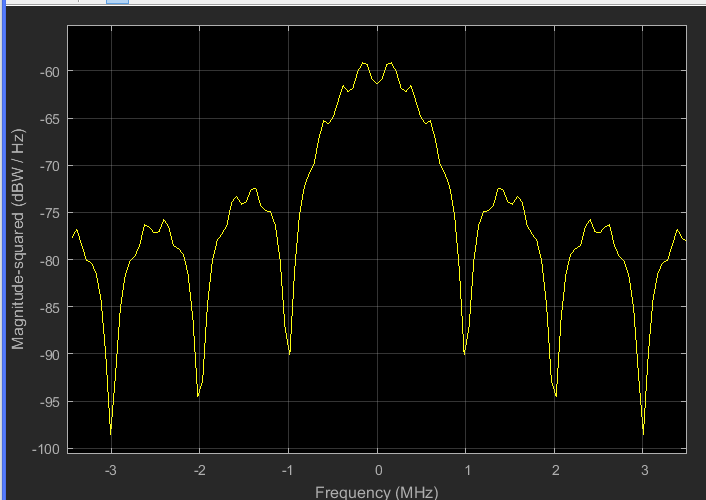
\includegraphics[width=0.78\linewidth]{spectren33}
\caption{spectre pour n = 3}
\label{fig:spectren33}
	\end{subfigure}
	~ %add desired spacing between images, e. g. ~, \quad, \qquad, \hfill etc. 
	%(or a blank line to force the subfigure onto a new line)
	\begin{subfigure}[b]{0.4\textwidth}
	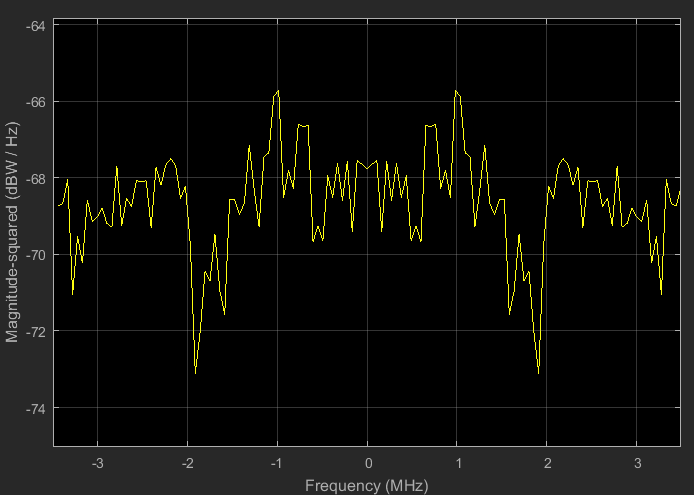
\includegraphics[width=0.78\linewidth]{spectren3}
\caption{spectre pour n = 3}
\label{fig:spectren3}
	\end{subfigure}
\end{figure}


\newpage
\section{Construction d'un récepteur}%3
L'opération de de-étalement effectuée au niveau du récepteur permet de retrouver notre signal
d'origine
\begin{figure}[h]
	\centering
	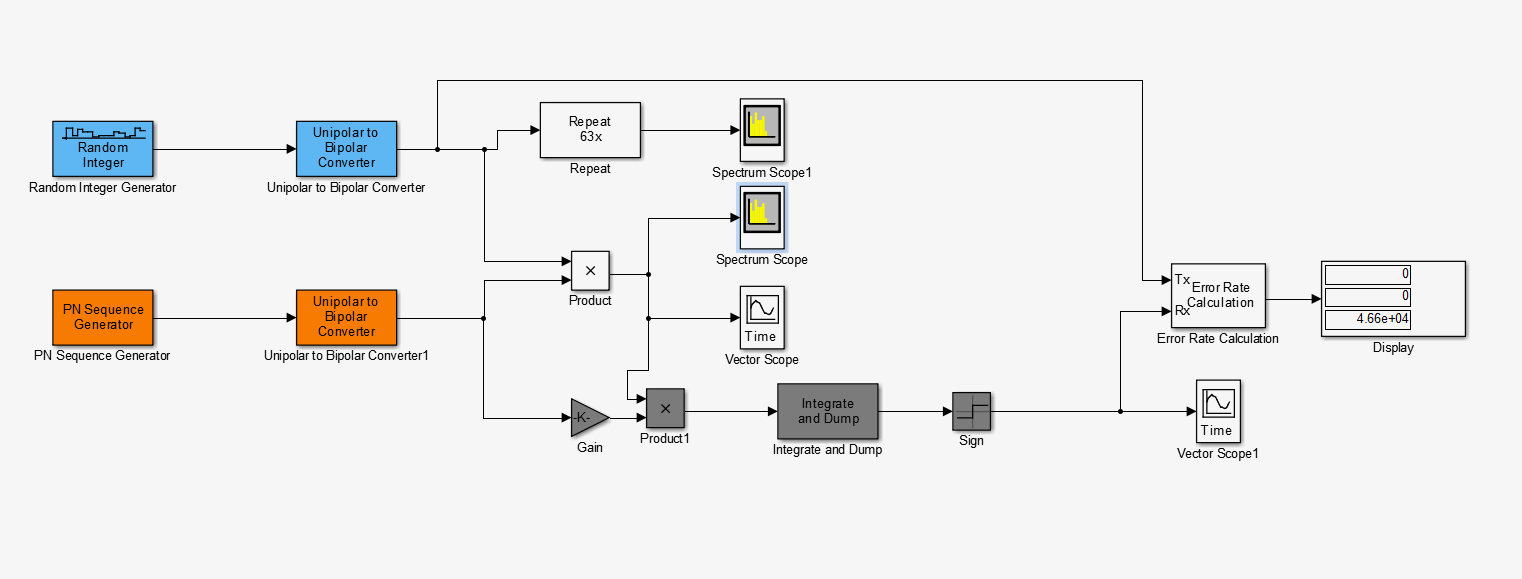
\includegraphics[width=0.7\linewidth]{schema_q1}
	\caption{shema q1}
	\label{fig:schemaq1}
\end{figure}

\begin{figure}[h]
	\centering
	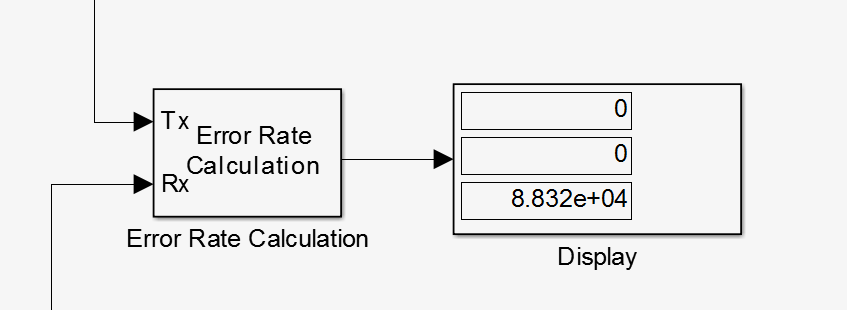
\includegraphics[width=0.7\linewidth]{error_q1}
	\caption{errror}
	\label{fig:errorq1}
\end{figure}




\newpage
\section{Analyse des codes}%4
%ESTO ESTA SUPER COPIADO CAMBIAR URGENTE
L'objectif de cette partie va être d'observer les fonctions d'inter et d'auto-correlation pour
différents codes utilisés dans les systèmes de communications numériques.
Dans cette section on a va démontrer l'orthogonalité des différentes codes. Cette propriété peût être vérifie par
le bias de la fonction d'intercorrelation qui vaut zero au proche à cette valeur quand les codes sont orthogonaux.\\
La fonction d'autocorrelation par contre caracterisera la capacité d'étalment du code.
%REESCRIBIR ESTO QUE ESTA COPIADO Y ADEMAS INVESTIGAR UN POCO
La fonction d'autocorrelation, caractérisera la capacité d'étalement du code, plus elle
sera proche de la réponse d'un bruit blanc (TF inverse d'une dsp constante sur toute la
bande : constante partout sauf dirac en zéro) meilleures seront ses performances en
terme d'étalement.


\subsection{Code Pseudo Aléatoire}
\begin{figure}[h]
	\centering
	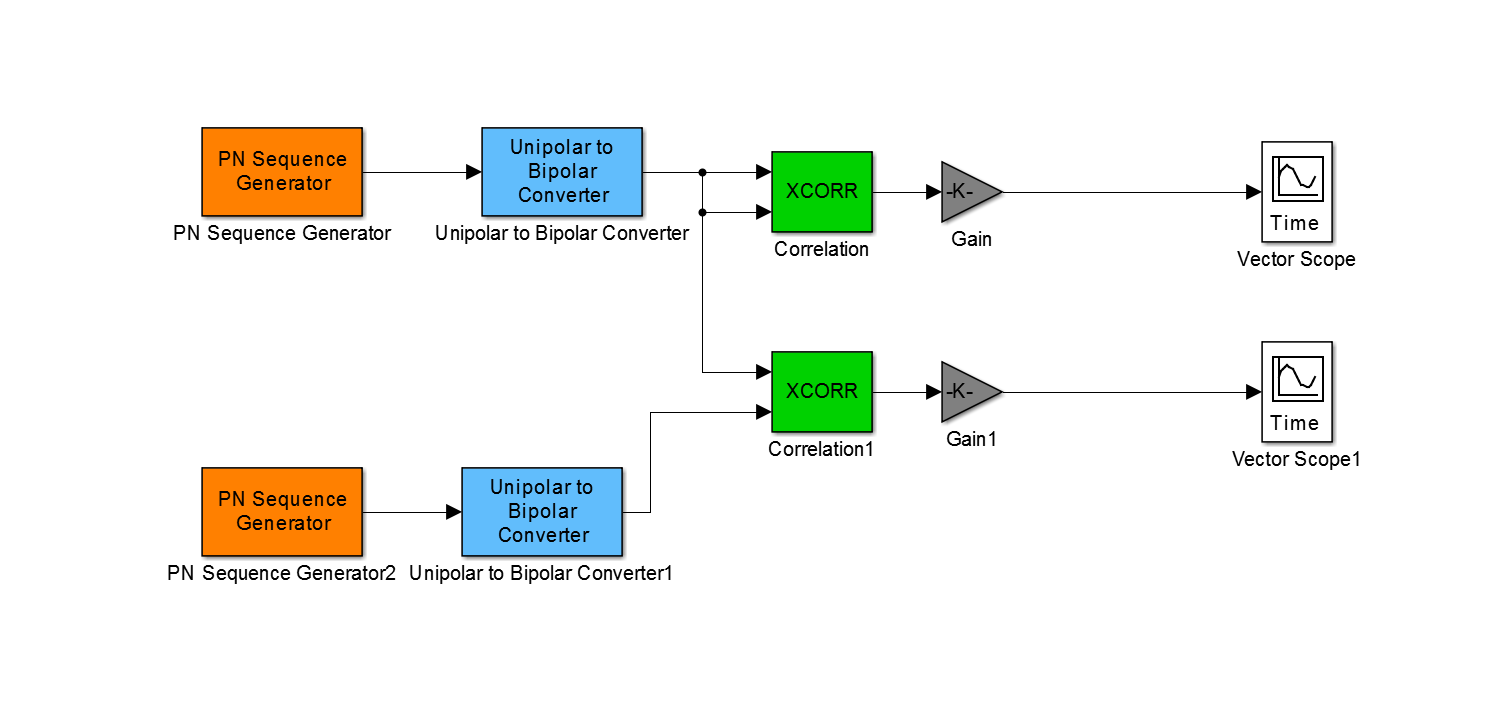
\includegraphics[width=0.7\linewidth]{schema_q2}
	\caption{schemq analysse code 1}
	\label{fig:schemaq2}
\end{figure}
 2 codes pseudo aléatoire "fils" de longueur 2 n -1 avec n = 7 ,
de polynômes générateurs différents et d'états initiaux différents.
\begin{figure}
	\centering
	\begin{subfigure}[b]{0.4\textwidth}
	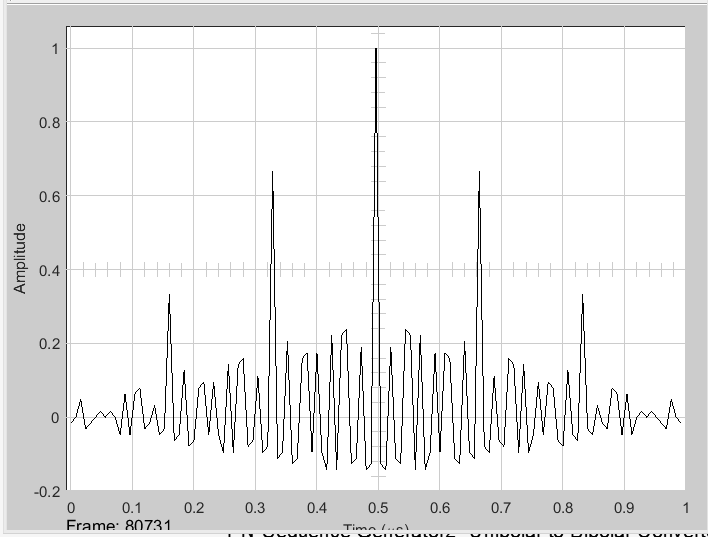
\includegraphics[width=0.7\linewidth]{codean1_altacorr}
\caption{altq correlqtion}
\label{fig:codean1altacorr}
	\end{subfigure}
	~ %add desired spacing between images, e. g. ~, \quad, \qquad, \hfill etc. 
	%(or a blank line to force the subfigure onto a new line)
	\begin{subfigure}[b]{0.4\textwidth}
	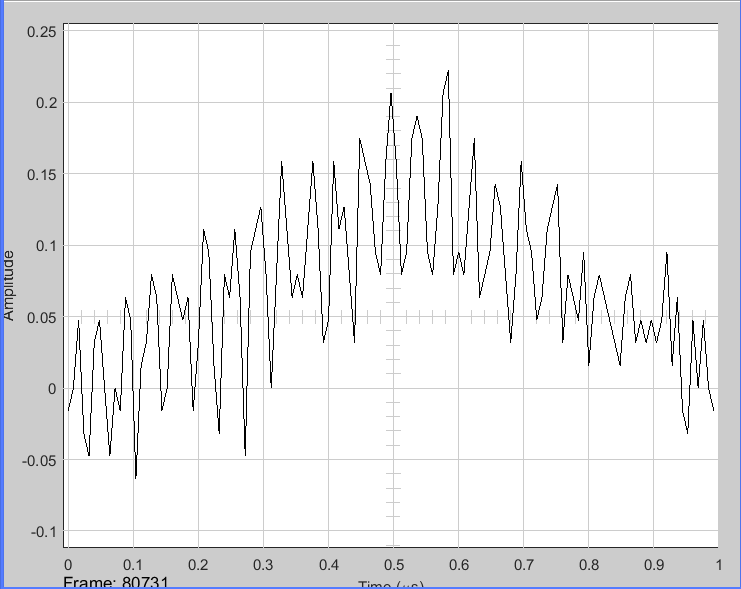
\includegraphics[width=0.7\linewidth]{codean1_bajacorr}
\caption{altq correlqtion}
\label{fig:codean1altacorr}
	\end{subfigure}
\end{figure}






%\begin{figure}[h]
%	\centering
%	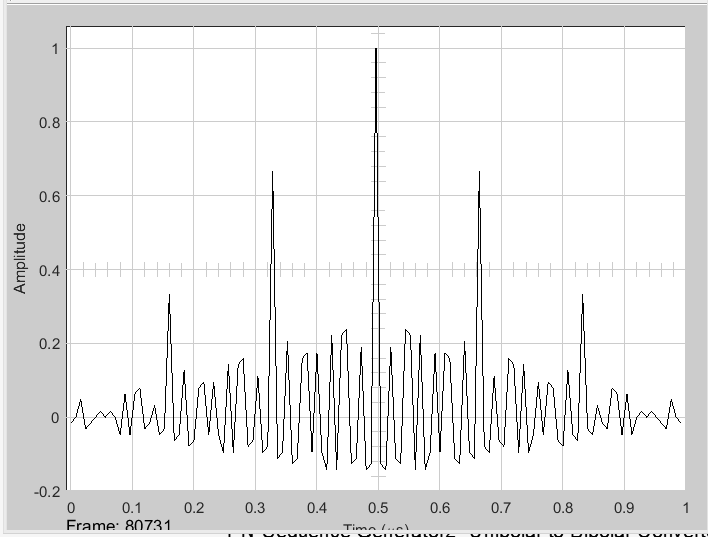
\includegraphics[width=0.7\linewidth]{codean1_altacorr}
%	\caption{altq correlqtion}
%	\label{fig:codean1altacorr}
%\end{figure}
%
%
%
%\begin{figure}[h]
%	\centering
%	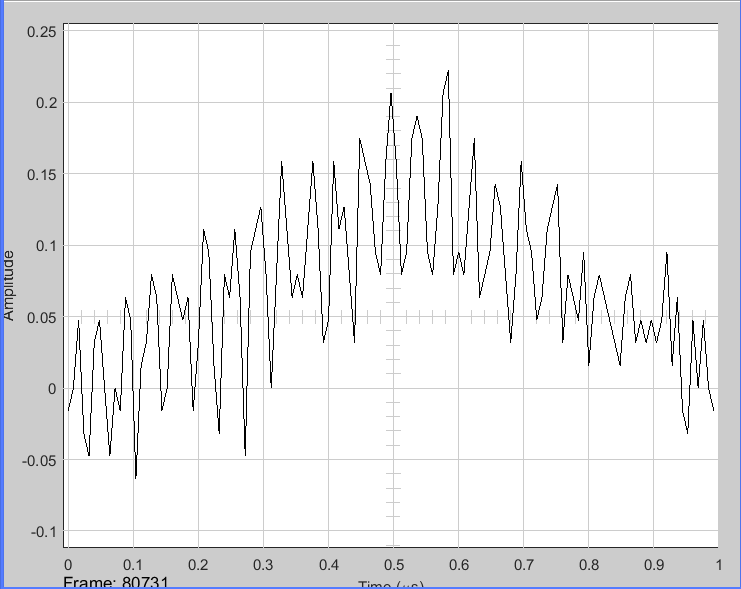
\includegraphics[width=0.7\linewidth]{codean1_bajacorr}
%	\caption{altq correlqtion}
%	\label{fig:codean1altacorr}
%\end{figure}

\newpage
\subsection{Hamard code}

\begin{figure}[t]
	\centering
	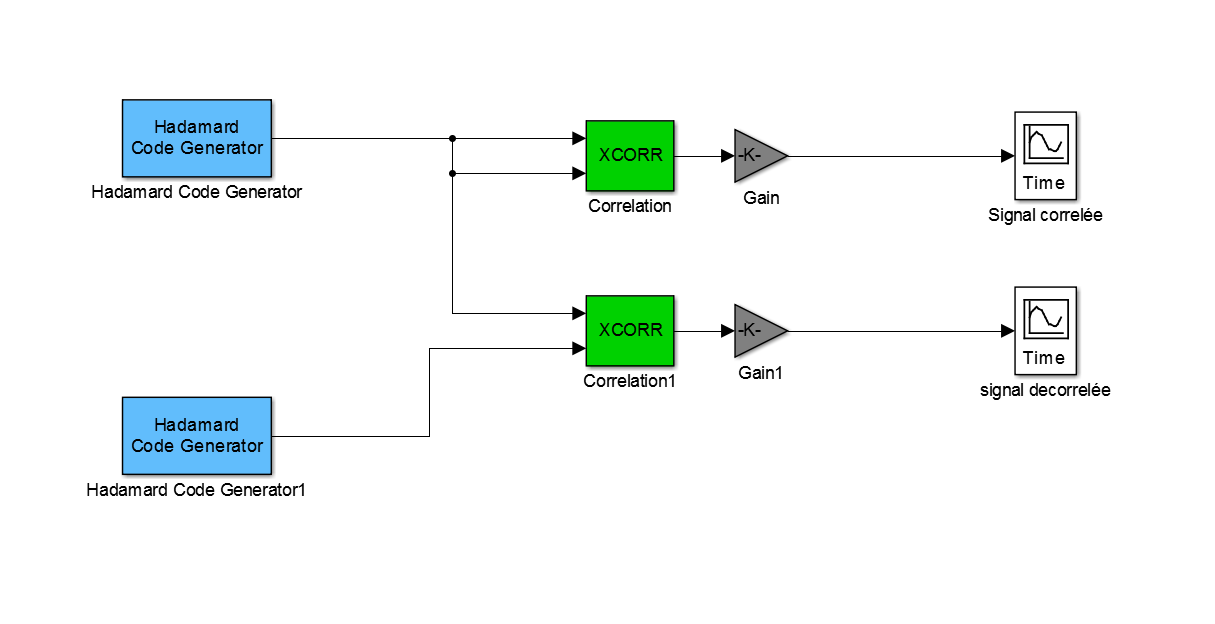
\includegraphics[width=0.7\linewidth]{schema_q2_analise_code_hamard}
	\caption{analise coce hamard schema}
	\label{fig:schemaq2analisecodehamard}
\end{figure}
Prendre un générateur de Hadamard " Hadamard Code Generator" [ code length : 128 ;
code index :% ∀; Tech=10 -6 /128 ; frame based output ; éch par trame = 128 ].
\begin{figure}[b]
	\centering
	\begin{subfigure}[b]{0.4\textwidth}
	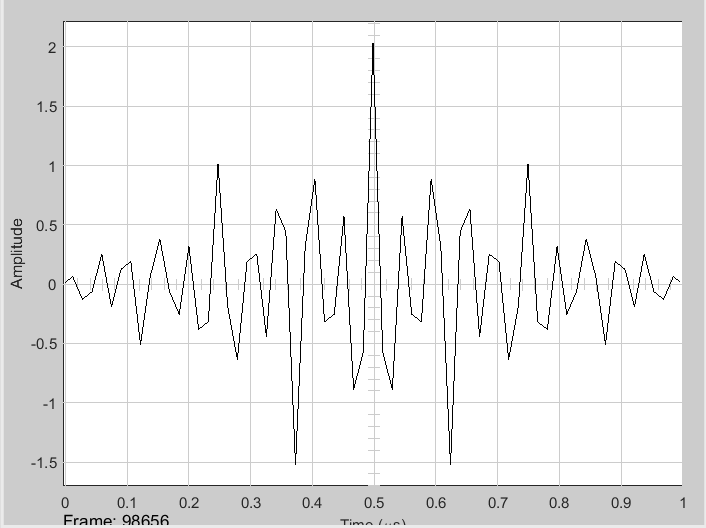
\includegraphics[width=0.7\linewidth]{hamard_altacorr}
\caption{}
\label{fig:hamardaltacorr}
	\end{subfigure}
	~ %add desired spacing between images, e. g. ~, \quad, \qquad, \hfill etc. 
	%(or a blank line to force the subfigure onto a new line)
	\begin{subfigure}[b]{0.4\textwidth}
	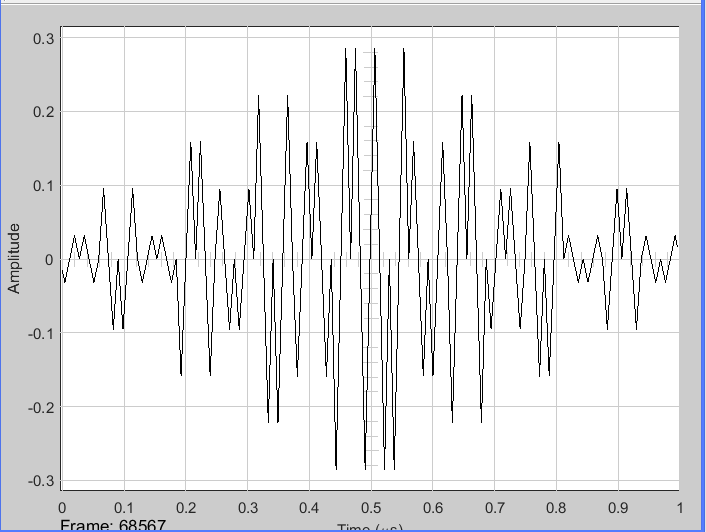
\includegraphics[width=0.7\linewidth]{hamard_bajacorr}
\caption{}
\label{fig:hamardbajacorr}
	\end{subfigure}
\end{figure}



%\begin{figure}[h]
%	\centering
%	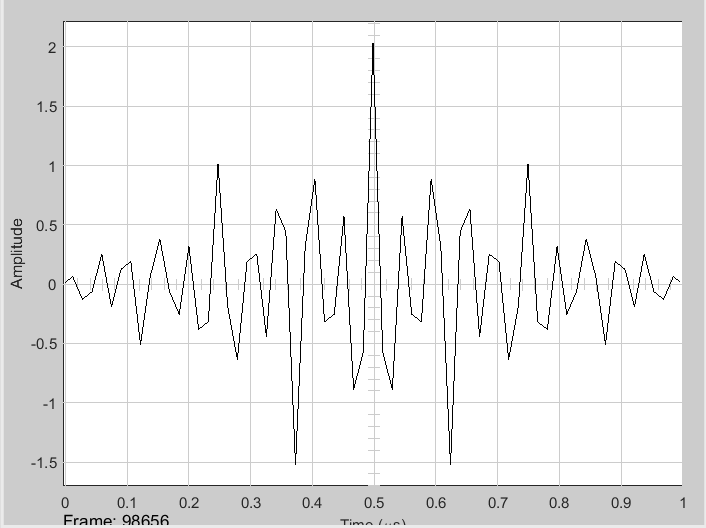
\includegraphics[width=0.7\linewidth]{hamard_altacorr}
%	\caption{}
%	\label{fig:hamardaltacorr}
%\end{figure}
%
%\begin{figure}[h]
%	\centering
%	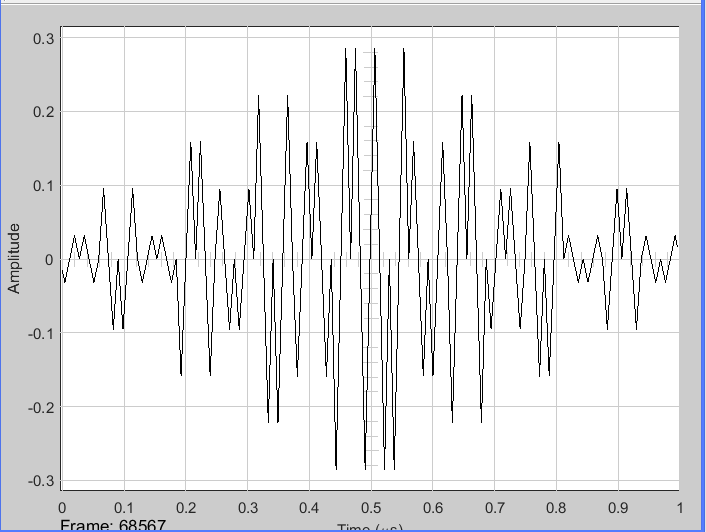
\includegraphics[width=0.7\linewidth]{hamard_bajacorr}
%	\caption{}
%	\label{fig:hamardbajacorr}
%\end{figure}

\newpage
\subsection{kasami code}
\begin{figure}[h]
	\centering
	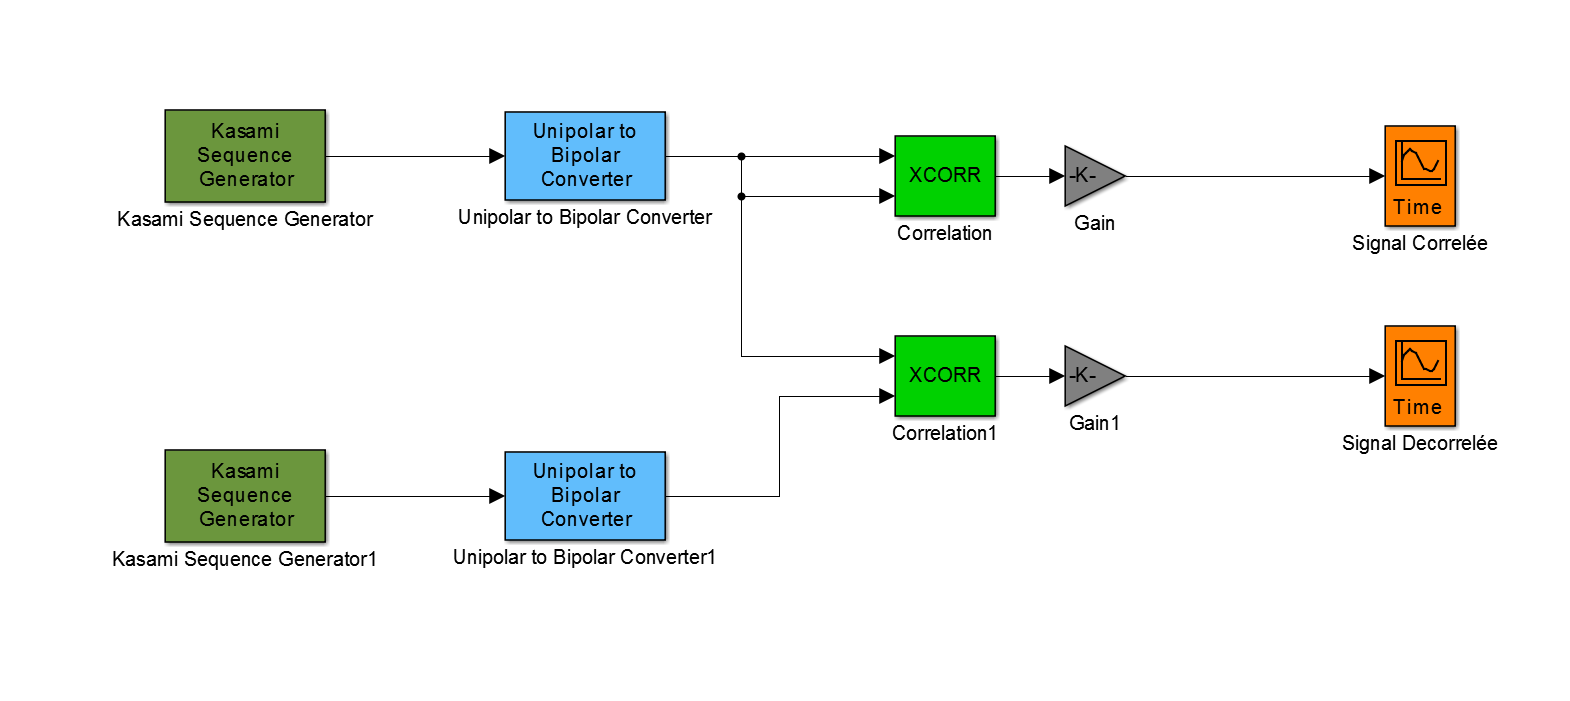
\includegraphics[width=0.7\linewidth]{schema_q2_analise_code_kasami}
	\caption{}
	\label{fig:schemaq2analisecodekasami}
\end{figure}

Faire l'auto et l'intercorrelation de 2 codes de Kasami "fils" de longueur 2 n -1 avec n = 6, de
polynômes générateurs identiques, d'états initiaux identiques mais d'indices différents.
\begin{figure}
	\centering
	\begin{subfigure}[b]{0.4\textwidth}
	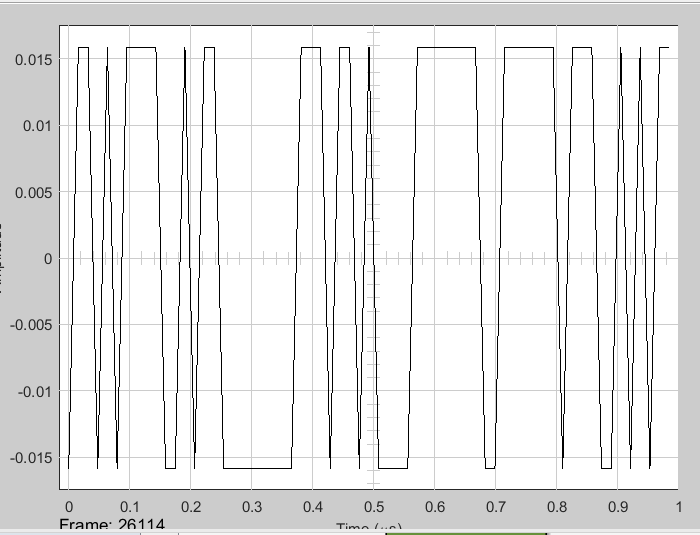
\includegraphics[width=0.7\linewidth]{kasami_bajacorr}
\caption{baja corr}
\label{fig:kasamibajacorr}
	\end{subfigure}
	~ %add desired spacing between images, e. g. ~, \quad, \qquad, \hfill etc. 
	%(or a blank line to force the subfigure onto a new line)
	\begin{subfigure}[b]{0.4\textwidth}
	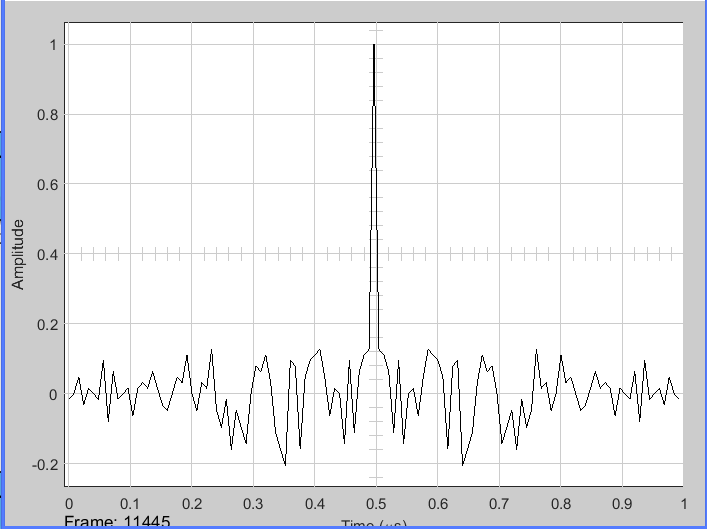
\includegraphics[width=0.7\linewidth]{kasami_altacorr}
\caption{alta corr}
\label{fig:kasamibajacorr}
	\end{subfigure}
\end{figure}




%
%\begin{figure}[h]
%	\centering
%	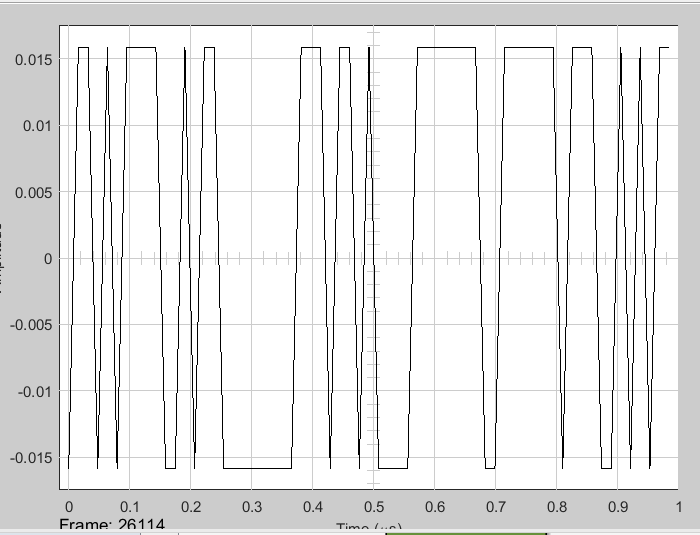
\includegraphics[width=0.7\linewidth]{kasami_bajacorr}
%	\caption{baja corr}
%	\label{fig:kasamibajacorr}
%\end{figure}
%\begin{figure}[h]
%	\centering
%	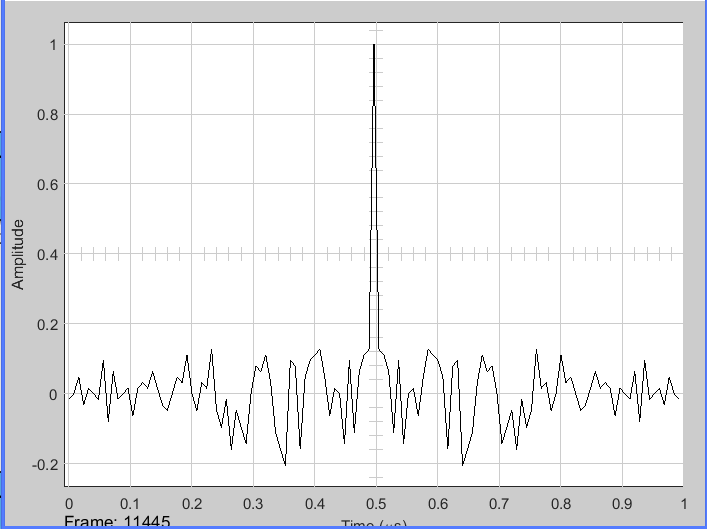
\includegraphics[width=0.7\linewidth]{kasami_altacorr}
%	\caption{alta corr}
%	\label{fig:kasamibajacorr}
%\end{figure}
%
\subsection{ lequel semble le plus adapté aux techniques d'accès CDMA ?}

La que tenga menos correlation
\chapter{Liaison CDMA}%5

Vous avez maintenant tous les éléments pour construire une liaison CDMA à 3 utilisateurs qui
utiliseront le même canal de transmission. Le canal de propagation sera simulé en mettant en
série
• un sommateur 3 voies
• un bruit blanc additif gaussien de puissance contrôlée.


%\section{Liaison montante : norme UMTS}%6





\section{Conclusions}










%------------------------------------------------------------------
% 	FIN
%-----------------------------------------------------------------



\end{document}























